\documentclass[tikz,border=2pt]{standalone}
\usepackage{tikz}
\usepackage{lmodern}
\usetikzlibrary{calc,decorations.pathreplacing}

% Visual conventions follow the existing MRNC TikZ pictures: ordinary
% components use TikZ's normal 0.4pt stroke, with compact TeX labels.
\tikzset{
  nu fibre/.style={
    x=0.78cm,
    y=0.78cm,
    line width=0.4pt,
    line cap=round,
    line join=round
  },
  nu label/.style={
    font=\scriptsize,
    inner sep=1pt
  },
  nu annotation/.style={
    font=\scriptsize,
    inner sep=1pt
  },
  nu dots/.style={
    font=\small,
    inner sep=0pt
  }
}


\begin{document}
% III-I_n^*-m

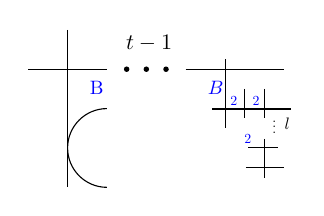
\begin{tikzpicture}[scale=0.5]
     \coordinate (C1) at (-1.50, 3.00);
  \coordinate (D1) at (-0.50, 3.00);
  \coordinate (A1) at (-1.00, 3.00);
  \coordinate (B1) at (-0.93, 3.26);

  \node[scale=0.8][above] at (B1) {$t-1$};
  \fill[black] (C1) circle (2pt);
  \fill[black] (D1) circle (2pt);
  \fill[black] (A1) circle (2pt);

  
  \coordinate (IIIrC) at (-4.00, 3.00);
  \coordinate (IIIrD) at (-2.00, 3.00);
  \coordinate (IIIrE) at (-3.00, 4.00);
  \coordinate (IIIrF) at (-3.00, 0.00);
  \coordinate (IIIrG) at (-2.00, 1.00);
  \coordinate (IIIrD_1) at (-2.26, 2.18);
  \draw (IIIrC) -- (IIIrD);
  \draw (IIIrE) -- (IIIrF);
  \draw (-2.00, 2.00) arc (90.0:270.0:1.00);
  \node[scale=0.7][above, text=blue] at (IIIrD_1) {B};


   \coordinate (G) at (0.76, 2.19);
  \coordinate (N) at (2.25, 1.25);
  \coordinate (O) at (2.58, 1.31);
  \coordinate (A) at (0.00, 3.00);
  \coordinate (B) at (2.50, 3.00);
  \coordinate (H) at (0.67, 1.99);
  \coordinate (I) at (2.67, 1.99);
  \coordinate (P) at (2.00, 1.23);
  \coordinate (Q) at (2.00, 0.23);
  \coordinate (R) at (1.59, 1.01);
  \coordinate (S) at (2.34, 1.01);
  \coordinate (T) at (1.53, 0.50);
  \coordinate (C) at (2.00, 2.50);
  \coordinate (D) at (2.00, 1.75);
  \coordinate (E) at (1.00, 3.25);
  \coordinate (F) at (1.00, 1.50);
  \coordinate (J) at (1.50, 2.50);
  \coordinate (K) at (1.50, 1.75);
  \coordinate (L) at (2.50, 0.50);
  \coordinate (M) at (1.22, 1.95);
  \coordinate (U) at (1.79, 1.95);
  \coordinate (V) at (1.58, 0.98);

  
  \node[scale=0.7][above, text=blue] at (G) {$B$};
  \node[scale=0.5][above] at (N) {$\vdots
$};
  \node[scale=0.6][above] at (O) {$l
$};
  \draw (A) -- (B);
  \draw (H) -- (I);
  \draw (P) -- (Q);
  \draw (R) -- (S);
  \draw (C) -- (D);
  \draw (E) -- (F);
  \draw (J) -- (J);
  \draw (J) -- (J);
  \draw (J) -- (K);
  \draw (T) -- (L);
  \node[scale=0.5][above, text=blue] at (M) {$2$};
  \node[scale=0.5][above, text=blue] at (U) {$2$};
  \node[scale=0.5][above, text=blue] at (V) {$2$};
\end{tikzpicture}

\end{document}
